\section{Related Works}
\label{sec:related_works}
\subsection{Video-Language Models}
Long-video understanding has attracted increasing attention in multimodal intelligence. Recent general-purpose MLLMs such as Gemini~\cite{gemini} and Long-VITA~\cite{longvita}, along with specialized video models including Video-XL~\cite{videoxl} and LongVLM~\cite{longvlm}, extend visual context to enable hour-scale video reasoning via uniform sampling. However, this paradigm faces a major bottleneck: limited context windows necessitate sparse sampling across the timeline, which can yield semantically redundant frames while simultaneously risking the loss of fleeting, query-critical cues. In parallel, contrastive video–language models~\cite{clip4clip} (e.g., Video-CLIP~\cite{videoclip}, X-CLIP~\cite{xclip}, and PE~\cite{perceptionenc}) extend CLIP-style contrastive embeddings to video, enabling query-conditioned retrieval of salient clips and frames. Nevertheless, contrastive objectives primarily optimize for semantic similarity and may miss cues that are implicitly relevant to the query intent but lack an explicit semantic match.

\begin{figure*}[t]
    \centering
    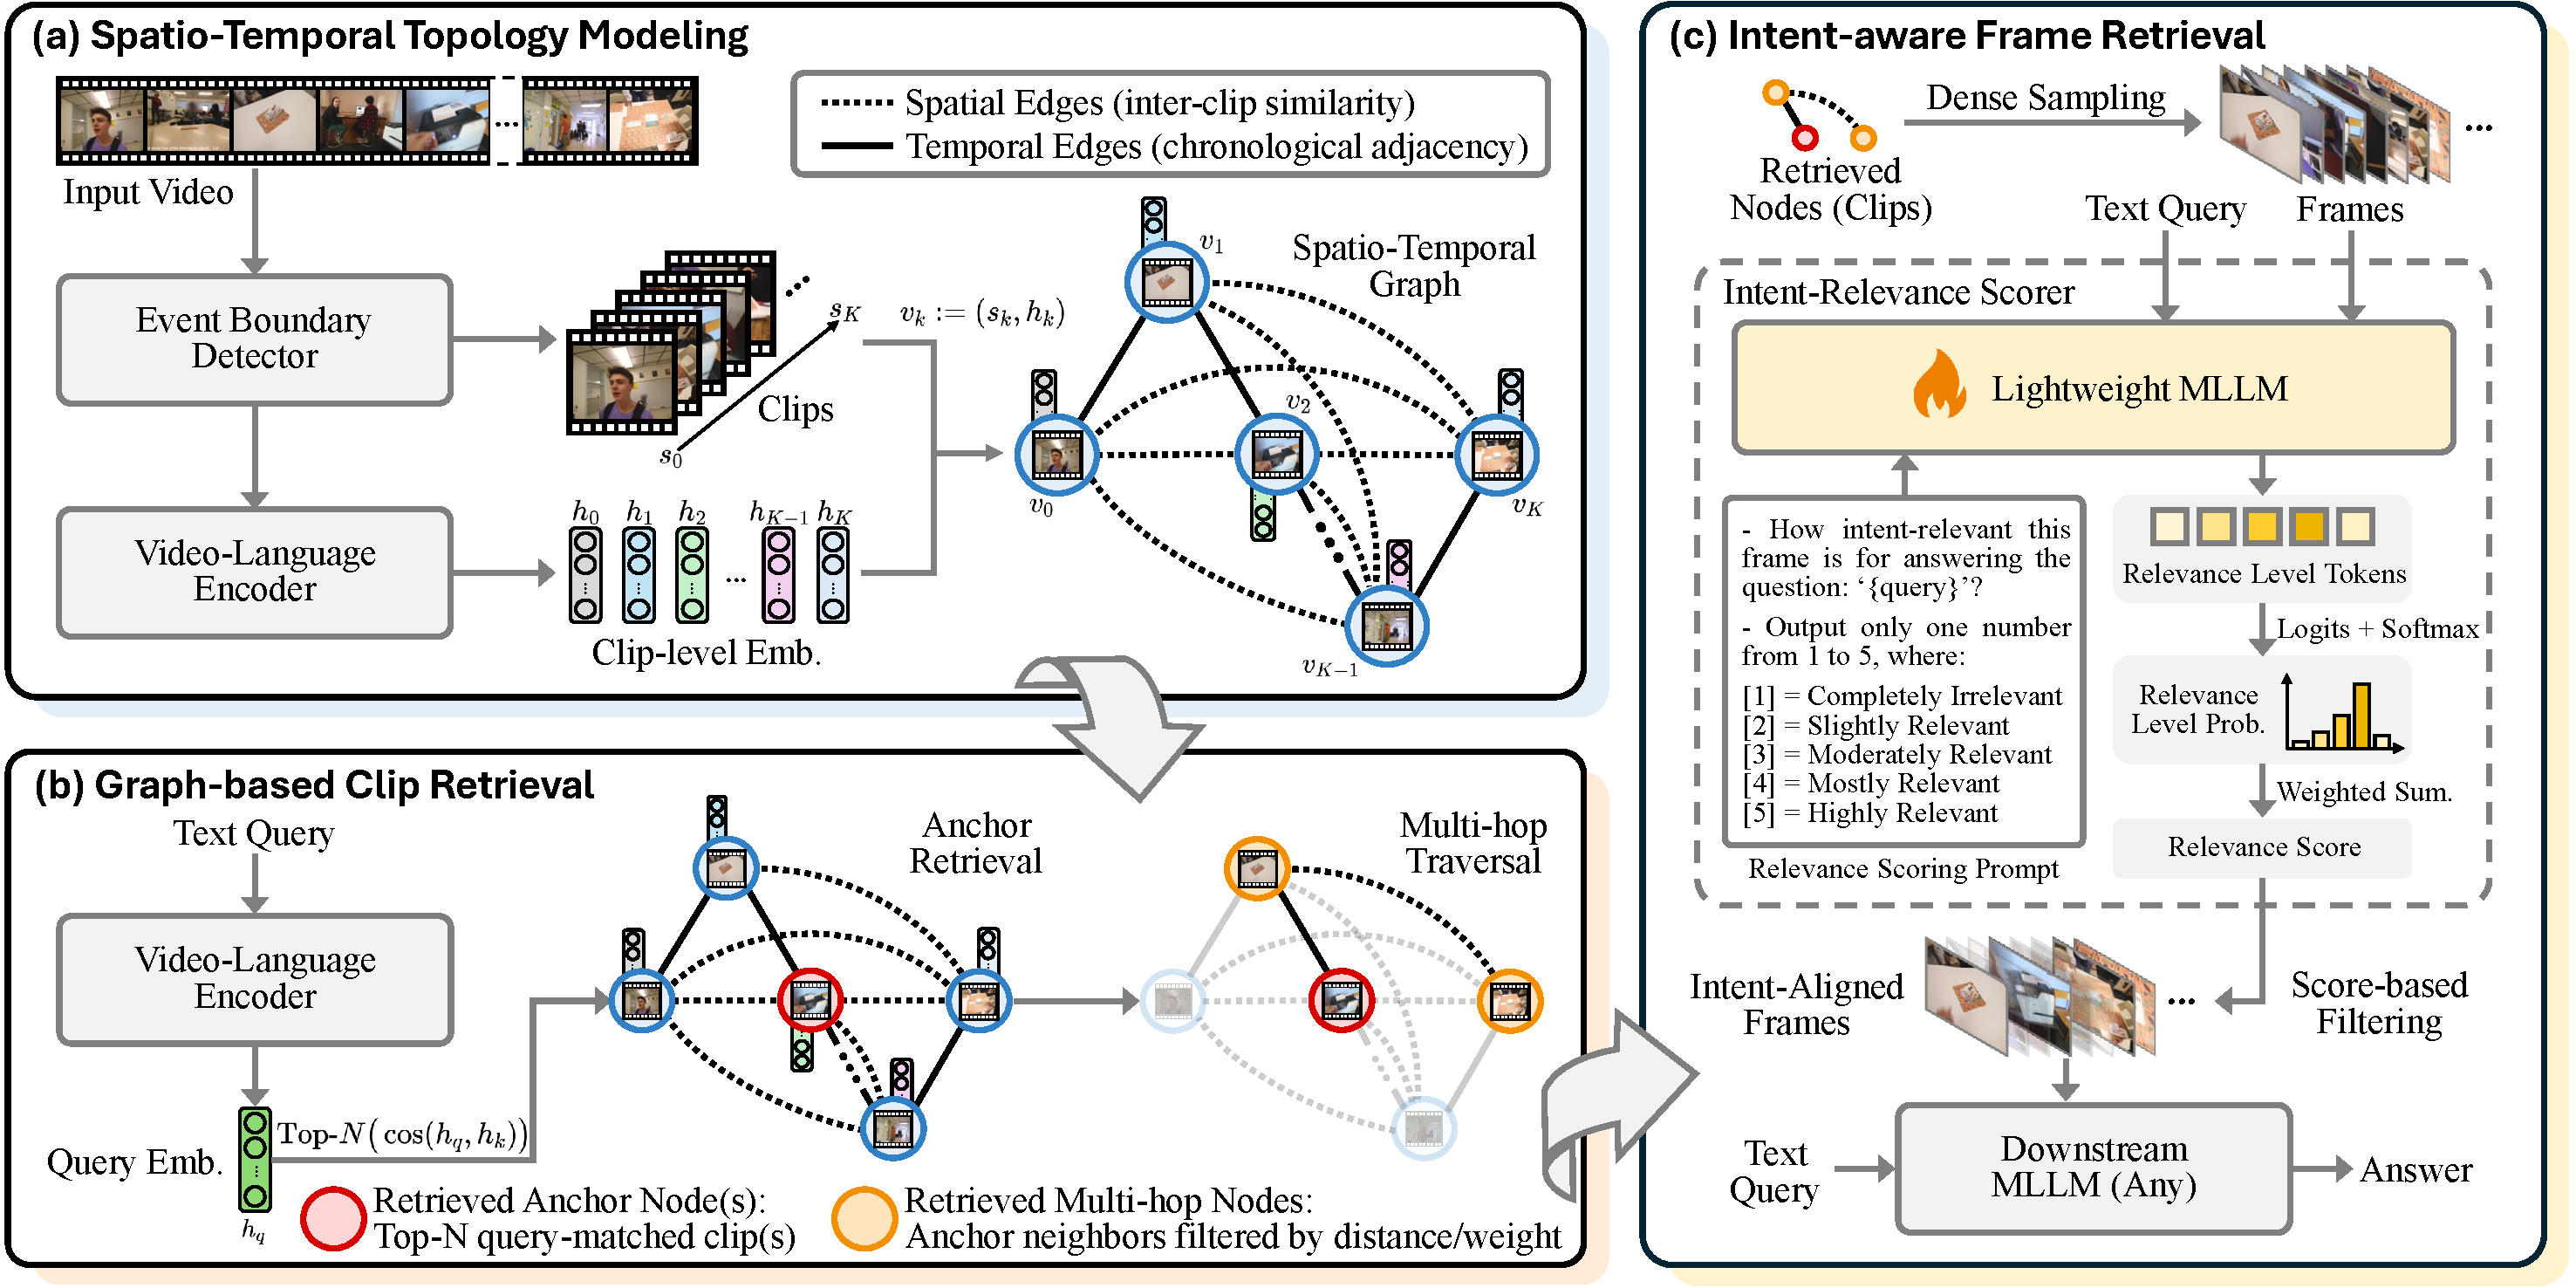
\includegraphics[width=\linewidth]{sec/figures/fw3.pdf}
    \caption{\small {\textbf{Overview of VideoStir.}} VideoStir achieves long-video understanding via spatio-temporal structuring and two-stage retrieval. \textbf{(a) Spatio-Temporal Topology Modeling.} An event boundary detector segments input video into semantically coherent clips. Their embeddings are used to construct a spatio-temporal graph with temporal edges linking adjacent clips and spatial edges weighted by inter-clip similarity. \textbf{(b) Graph-based Clip Retrieval}. Input query is embedded in the video-language space to retrieve top-$N$ matched anchor nodes; multi-hop traversal then expands along spatio-temporal links under hop-distance and edge-weight constraints to aggregate contextual clips. \textbf{(c) Intent-aware Frame Retrieval.} Frames densely sampled from the retrieved clips are assessed by an intent-relevance scorer (LoRA-tuned on IR-600K), which outputs a probability distribution over discrete relevance levels. These distributions are then aggregated via probability-weighted expectation to produce a continuous relevance score; high-scoring, intent-aligned frames are retained and fed to a downstream MLLM to produce the final answer.}
    \label{fig:fw}
    % \vspace{-0.10in}
\end{figure*}


\subsection{Agentic Long-Video Understanding}
To alleviate the contextual intractability inherent in processing long-duration videos, a growing body of recent work has shifted towards leveraging external systems. These systems are designed to reconstruct and distill extensive long-range context into compact, semantically rich cues tailored for downstream MLLMs. A prominent trajectory within this domain involves the exploration of agentic frameworks~\cite{mmvid,omagent}, which employ (M)LLMs as decision-making policies equipped with advanced modules for captioning, multi-step reasoning, and external memory~\cite{VideoMem}. By simulating human-like curation processes~\cite{vamos,morevqa}, these agents dynamically filter irrelevant data. For example, DrVideo~\cite{drvideo} synthesizes disjoint video frames into coherent long-form textual narratives to facilitate precise query answering, while Vgent~\cite{vgent} abstracts complex entity interactions into structured symbolic representations to bolster reasoning. However, despite their demonstrated efficacy in enhancing understanding, deploying such sophisticated MLLM-based policies incurs substantial inference overhead.

\subsection{RAG for Long-Video Understanding}
{To reduce the procedural inference overhead of agentic workflows, another line of work explores long-video retrieval-augmented generation (RAG) frameworks~\cite{exvideorag,xue2025omni,zeng2025scenerag}, which externally select cues to fit limited context windows~\cite{videorag,TVRAG,FOCUS}. For example, Video-RAG~\cite{Video-RAG} retrieves keyframes via semantic similarity, and enriches entity information with external tools like optical character recognition and object detectors. E-VRAG~\cite{evrag} introduces a retrieval-reranking pipeline, leveraging Qwen3-Reranker-style binary judgments for fine-grained selection. while AKS~\cite{AKS} selects keyframes by jointly optimizing query-frame semantic similarity and temporal uniformity. However, existing methods often treat videos as independent segments, decoupling intrinsic spatio-temporal structure and limiting coherent reasoning. Moreover, current paradigms favor explicit semantic matching over intent-level alignment, risking the omission of cues implicitly relevant to the query intent.}

% \subsection{Intent-aware ...} %多模态领域还没有，可以说推荐系统的策略 
% Rerankers serve as a crucial second stage in recent advanced RAG systems, refining initially retrieved candidates to provide more precise and causally aligned contexts for generation~\cite{MonoT5}. In the text domain, rerankers such as Qwen3-Reranker~\cite{Qwen3} and BGE-Reranker~\cite{bge_m3} effectively reorder documents based on intent-level relevance estimation. In the multimodal domain~\cite{chen2024mllm}, models like MM-R5~\cite{mmr5} and MonoQwen~\cite{MonoQwen} have preliminarily extended this idea to image–text retrieval. These works demonstrate that retrieval–reranking architectures can significantly improve retrieval quality compared with purely similarity-based retrieval. However, existing multimodal rerankers trained on static image–text pairs perform poorly when distinguishing densely similar and continuous video frames. To bridge this gap, we curate the IR-600K dataset and develop a frame reranker tailored for long-video RAG, enabling intent-aware and causally aligned frame selection, and establishing a foundation for advanced retrieval–reranking architectures in long-video understanding systems.

% %MonoQwen应该是做多模态文档检索的，现有的工作trained on文档检索任务无法直接迁移到....
